%!TEX root = ../rapport.tex
%!TEX encoding = UTF-8 Unicode

% Chapitres "Introduction"

% modifié par Francis Valois, Université Laval
% 31/01/2011 - version 1.0 - Création du document


\label{s:experimentation}
\chapter{Laboratoire 2}
\section{Projet 1}
Nous avons choisi une charge de valeur 100$\Omega$ puisque pour cette valeur, on obtient un coefficient de réflexion théorique faible. Pour affirmer cela, on utilise l'expression suivante:
\begin{equation}
\Gamma_g (s) = \frac{Z_g(s) - Z_0(s)}{Z_g(s) + Z_0(s)}\label{eq:reflex}
 \end{equation} 

\paragraph{}Dans le circuit étudié, on cherche à avoir $Z_0$ (l'impédance mise en parallèle avec la source) $\approx Z_G$ (l'impédance de la ligne)

\paragraph{}Afin d'observer de manière pratique le comportement des réflexions du circuit, nous avons essayé chacune des résistance disponible dans les choix en plus de celle de 100$\Omega$. Nous présenterons les courbes obtenus à l'oscilloscope à l'annexe \ref{s:annexes}. Comme seule la courbe pour la résistance de 100$\Omega$ est requise selon l'énoncé de laboratoire, elle est présentée ci-dessous:

\begin{figure}[htb]
\begin{center}
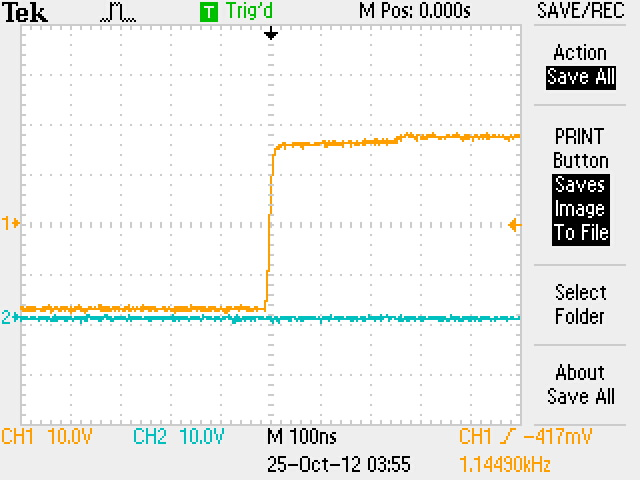
\includegraphics[scale=0.3]{Reflexion_R_100.jpg}
\caption{Courbes obtenus à l'oscilloscope pour le projet 1 en utilisant une résistance de 100 $\Omega$}
\label{Reflexion_R_100}
\end{center}
\end{figure}

On note dans cette figure que la réflexion est bel et bien faible, mais existante, en utilisant une résistance variable (le potentiomètre), on lit au multimètre une résistance très proche de 93$\Omega$. Cette résistance est très proche de l'impédance intrinsèque de ligne du tableau 1 présenté dans le protocle de laboratoire( $z_0 = 93\Omega$). L'ensemble des autres courbes est présenté dans l'annexe \ref{s:annexes}

\paragraph{}On remarque que la valeur fournie par le manufacturier est très précise. La différence entre la valeur du manufacturier et celle mesurée repose sur le bruit du signal qui affecte la précision de la lecture à l'oscilloscope et aussi la précision limitée de l'instrument de mesure de la résistance. 

\paragraph{}Pour ce qui est de déterminer la longueur de ligne, nous avons que la première réflexion vue à la source pour une résistance de 27 $\Omega$ est vue à une différence de temps (par rapport à la montée initiale) de $\approx 250ns$. Or, ce temps correspond au temps d'aller-retour. Afin de déterminer la longueur de la ligne, on divise par deux le temps d'aller-retour, ce qui donne 125ns et puis, on divise la vitesse de propagation par ce temps. Soit $v_p = 0.86 \times c \left[\frac{m}{s}\right]$, $l \left[m\right] = 0.86\times c \left[\frac{m}{s}\right] \times 125 ns = 37.475 \left[m\right]$. La ligne de transmission fait donc 37.475$\left[m\right]$ de long.

\section{Projet 2}

Dans ce projet, il était demandé de visualiser simultanément les signaux au niveau de la charge et de la source sur la ligne RG-58 de 30m. Cela fut fait pour des charges de respectivement 0 $\Omega$, 27 $\Omega$ et 50$\Omega$. Les courbes obtenues sont présentées à la section suivante.
\subsection{Présentation des courbes obtenues expérimentalement}
\begin{figure}[htb]
	\centering
\subfigure[Régime transitoire pour $R = 0 \Omega$]{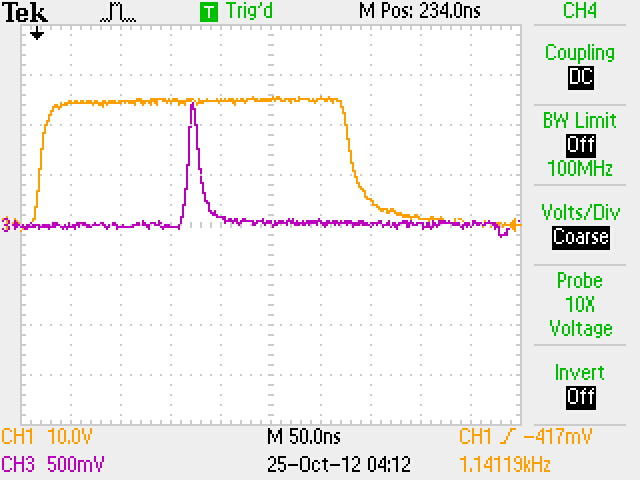
\includegraphics[scale =0.3]{fig/TR0.JPG} \label{fig:transr0}}
		\quad
		\subfigure[Front montant du régime transitoire pour $R = 27 \Omega$]{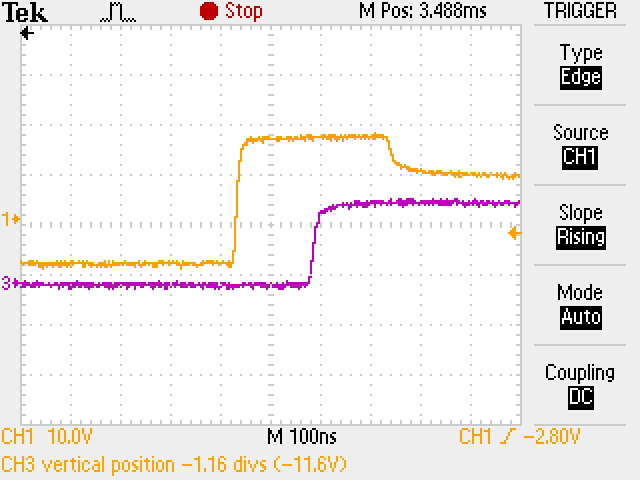
\includegraphics[scale =0.3]{fig/TR272.JPG} \label{fig:transr272}}
		\quad
		\subfigure[Front descendant du régime transitoire pour $R = 27 \Omega$]{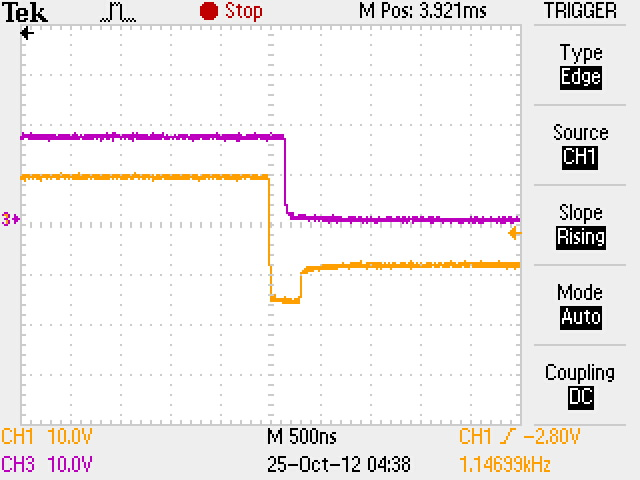
\includegraphics[scale =0.3]{fig/TR271.JPG} \label{fig:transr271}}
		\quad
		\subfigure[Vue d'ensemble du régime transitoire pour $R = 27 \Omega$]{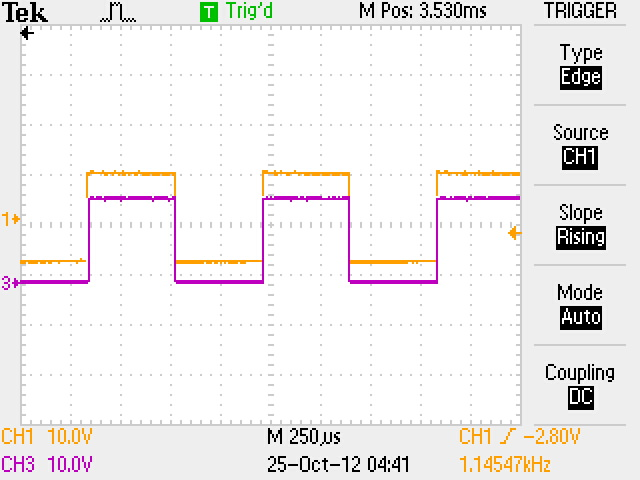
\includegraphics[scale =0.3]{fig/TR273.JPG} \label{fig:transr273}}
\end{figure}

\setcounter{subfigure}{0}
\begin{figure}[htb]
	\centering
\subfigure[Front montant du régime transitoire pour $R = 50 \Omega$]{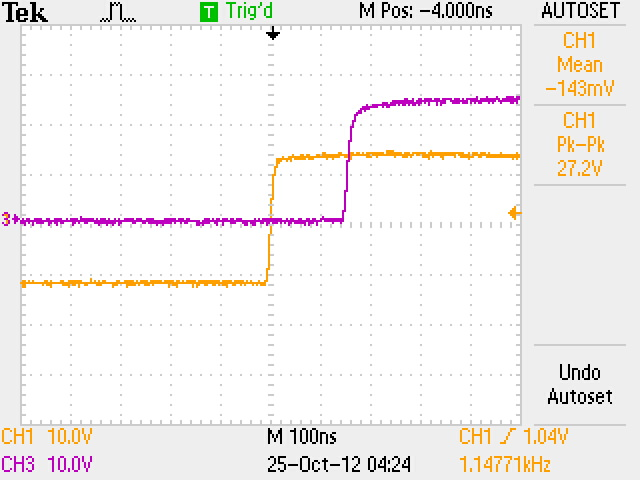
\includegraphics[scale =0.3]{fig/TR501.JPG} \label{fig:transr501}}
		\quad
		\subfigure[Front descendant du régime transitoire pour $R = 50 \Omega$]{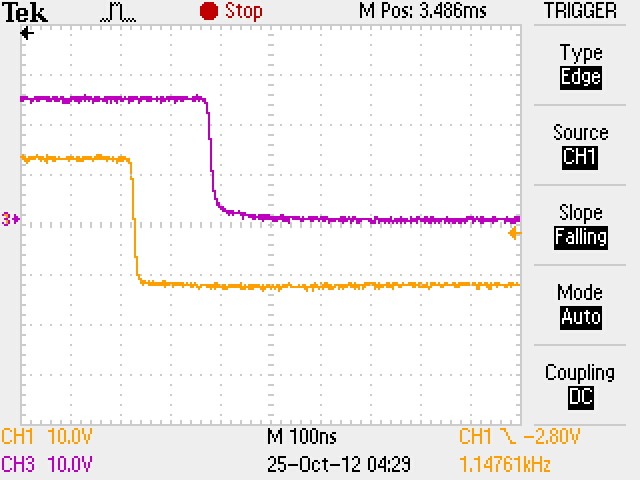
\includegraphics[scale =0.3]{fig/TR502.JPG} \label{fig:transr502}}
		\quad
		\subfigure[Vue d'ensemble du régime transitoire pour $R = 50 \Omega$]{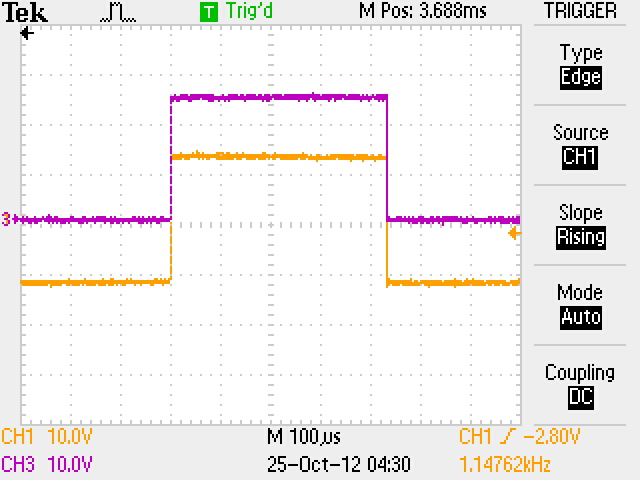
\includegraphics[scale =0.3]{fig/TR503.JPG} \label{fig:transr503}}
\end{figure}
\newpage
\subsection{Présentation des calculs}
Un example de chacun des calculs demandés est présenté ci-dessous.
L'équation utile au calcul du coefficient de réflexion est présentée à l'équation \ref{eq:reflex}. 
\subsubsection*{Calcul du coefficient de réflexion vu par la source}
Le développement du calcul du coefficient de réflexion vu par la source est présenté ci-dessous:
\begin{align}
\Gamma_g (s) &= \frac{Z_g(s) - Z_0(s)}{Z_g(s) + Z_0(s)}\\
		 &= \frac{50 - 50 }{50 + 50}\notag\\
		 &= 0\notag
\end{align}
\subsubsection*{Calcul de la tension $V^{+}(s)$}
On note premièrement sur la figure \ref{fig:transr501} que la tension de la source était de 27.2 V.
\begin{align}
V^{+}(s) &=  \frac{Z_0}{Z_0 + R_g} V_g (s)\\
		 &=	 \frac{50}{50 + 50} 27.2 \notag\\
		 &=  13.6V\notag
\end{align}

\subsubsection*{Calcul des coefficients de réflexion vus aux charges}
\begin{equation}
\Gamma_c (s) = \frac{Z_c(s) - Z_0(s)}{Z_c(s) + Z_0(s)}
\end{equation}
\textbf{Pour R = $0\Omega$}
\begin{align*}
\Gamma_c (s) &= \frac{Z_c(s) - Z_0(s)}{Z_c(s) + Z_0(s)}\\
			 &= \frac{0 - 50 }{0 + 50}\\
			 &= -1
\end{align*}
\textbf{Pour R = $27\Omega$}
\begin{align*}
\Gamma_c (s) &= \frac{Z_c(s) - Z_0(s)}{Z_c(s) + Z_0(s)}\\
			 &= \frac{27 - 50 }{27 + 50}\\
			 &= -0.2987
\end{align*}
\textbf{Pour R = $50\Omega$}
\begin{align*}
\Gamma_c (s) &= \frac{Z_c(s) - Z_0(s)}{Z_c(s) + Z_0(s)}\\
			 &= \frac{50 - 50 }{50 + 50}\\
			 &= 0
\end{align*}
\newpage
\subsection{Présentation des courbes théoriques}
Les courbes théoriques utiles pour l'analyse et la discussion sont présentées ci-dessous.
\setcounter{subfigure}{0}
\begin{figure}[htb]
	\centering
\subfigure[Régime transitoire théorique pour $R = 0 \Omega$]{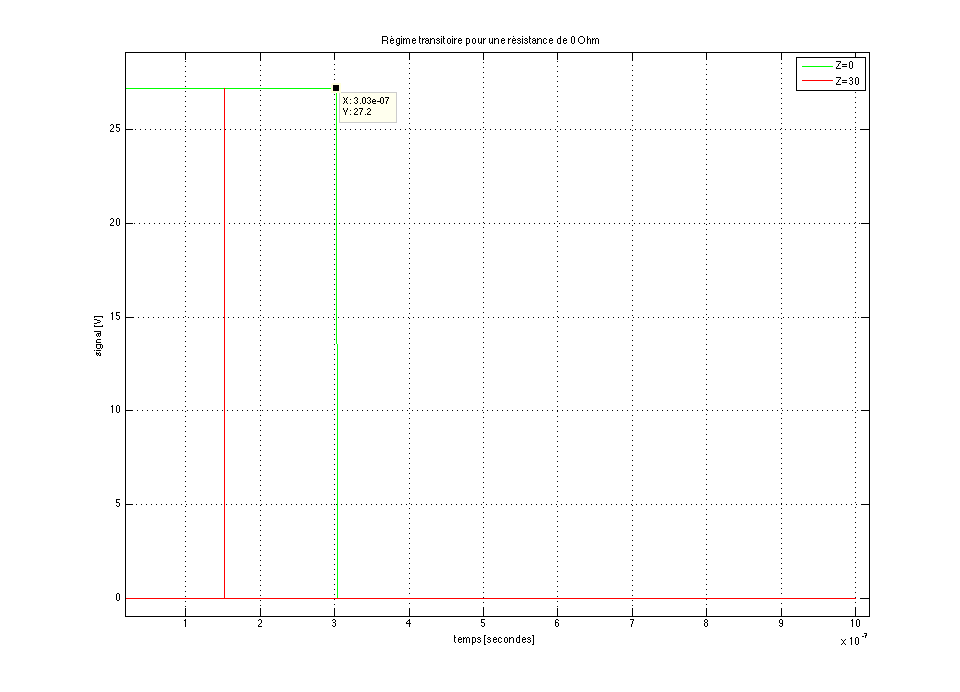
\includegraphics[scale =0.2]{fig/r0.png} \label{fig:r0}}
		\quad
		\subfigure[Régime transitoire théorique pour $R = 27 \Omega$]{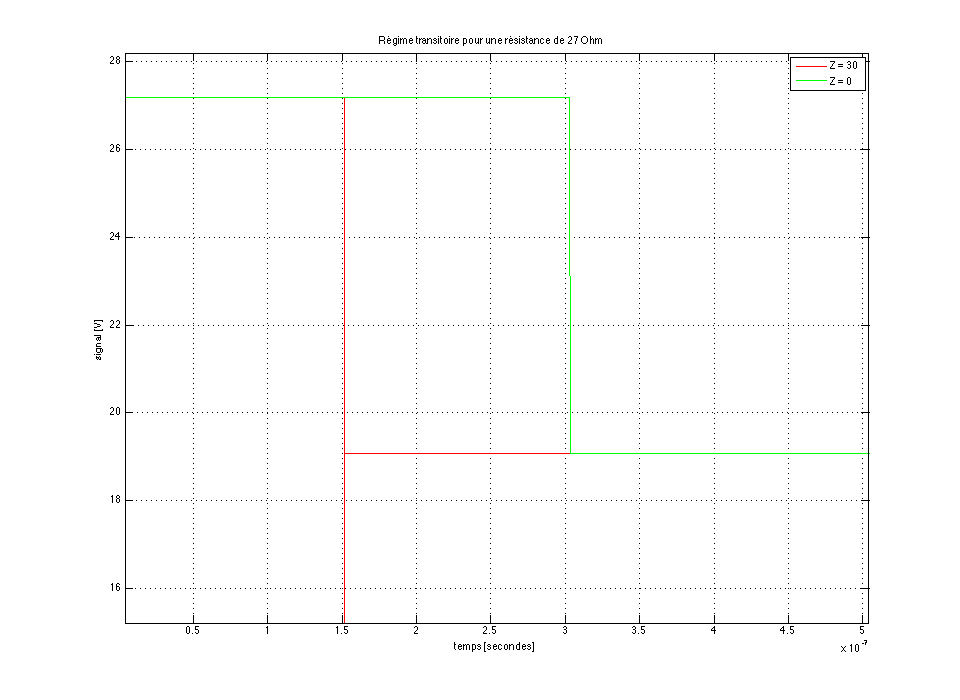
\includegraphics[scale =0.2]{fig/r27.png} \label{fig:r27}}
		\quad
		\subfigure[Régime transitoire théorique pour $R = 50 \Omega$]{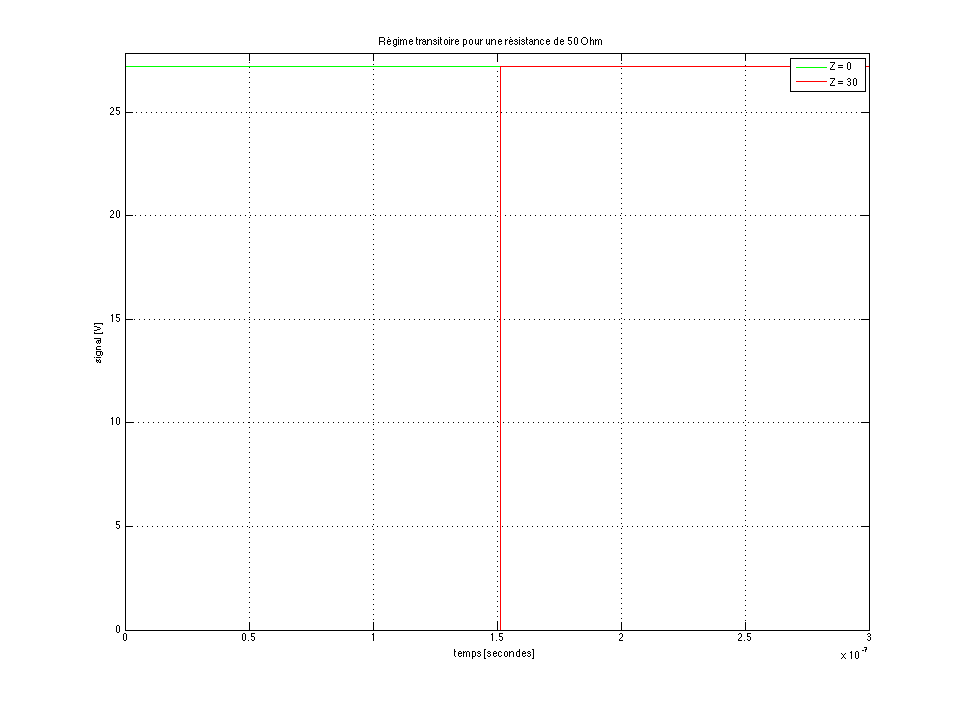
\includegraphics[scale =0.2]{fig/r50.png} \label{fig:r50}}
\end{figure}


\newpage
\setcounter{subfigure}{0}
\begin{figure}[htb]
	\centering
\subfigure[Diagramme en z pour $R = 0 \Omega$]{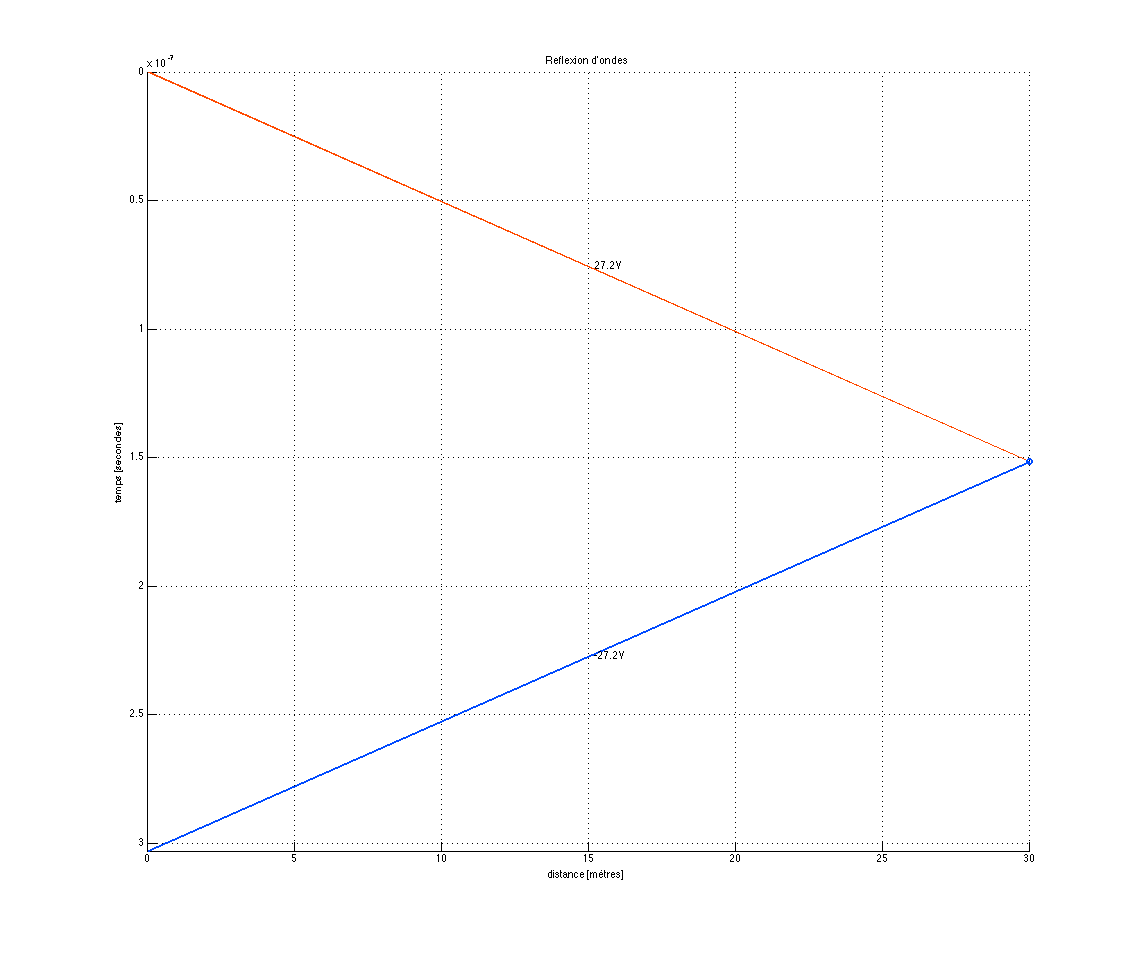
\includegraphics[scale =0.15]{fig/zr0.png} \label{fig:zr0}}
		\quad
		\subfigure[[Diagramme en z pour $R = 27 \Omega$]{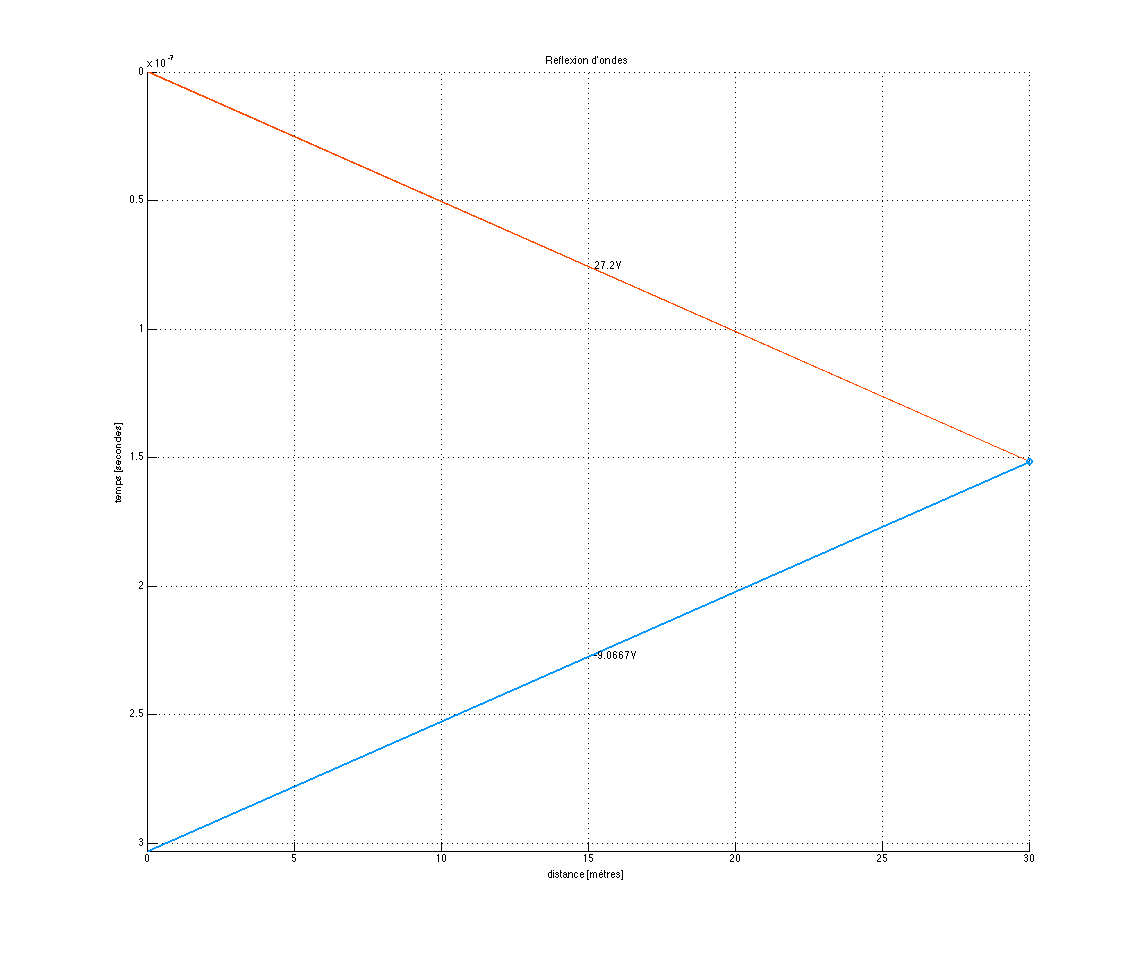
\includegraphics[scale =0.15]{fig/zr25.png} \label{fig:zr25}}
		\quad
		\subfigure[[Diagramme en z pour $R = 50 \Omega$]{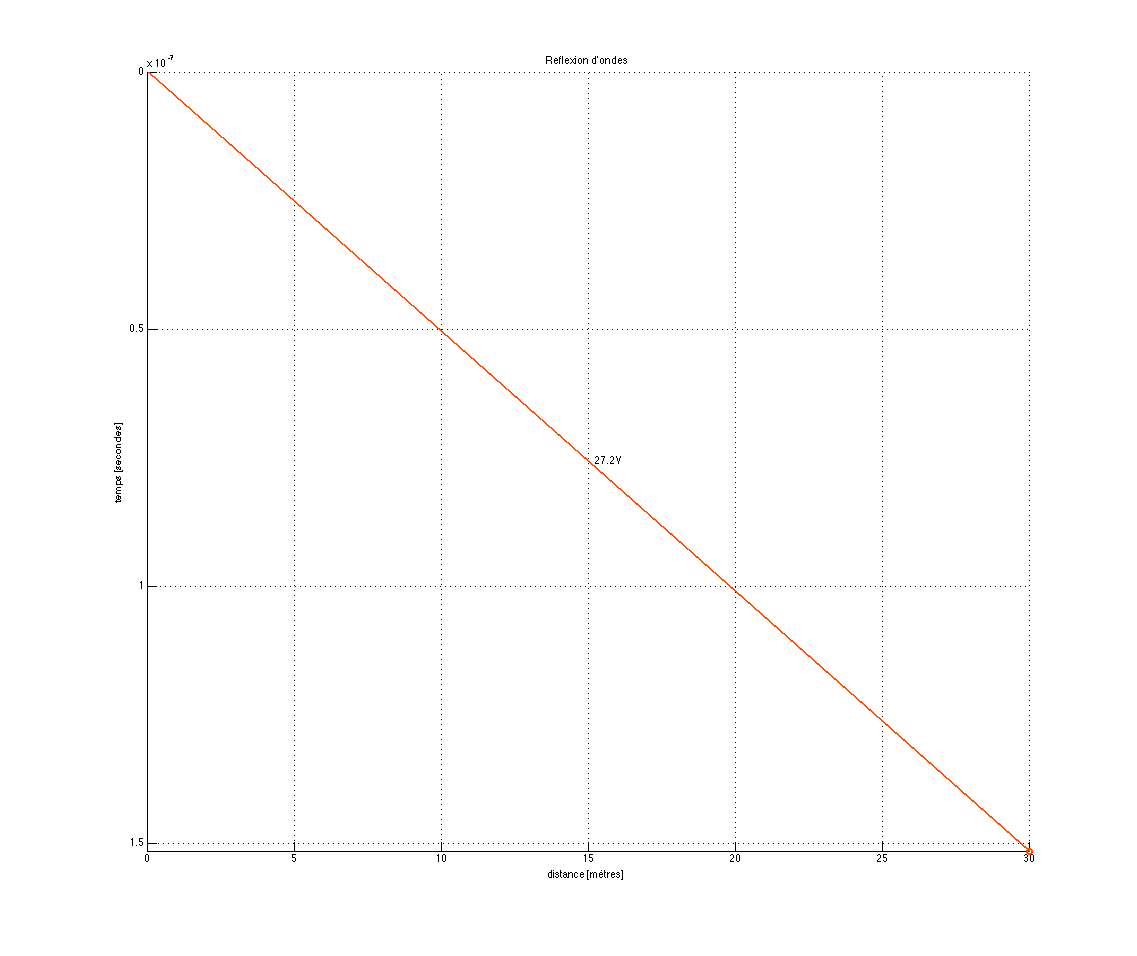
\includegraphics[scale =0.15]{fig/zr50.png} \label{fig:zr50}}
\end{figure}
\clearpage
\newpage
\subsection{Discussion}
\clearpage
\newpage
\section{Projet 3}
La courbe observée à l'oscilloscope est présentée à la figure \ref{CC2}. Le numéro de la charge utilisée est TOEM \#1. On identifie graphiquement une forme de courbe $R-L$ série.  Le $V^{+}$  est de 14V et le 2$V^{+}$ d'environ 27V.

\begin{figure}[htb]
\begin{center}
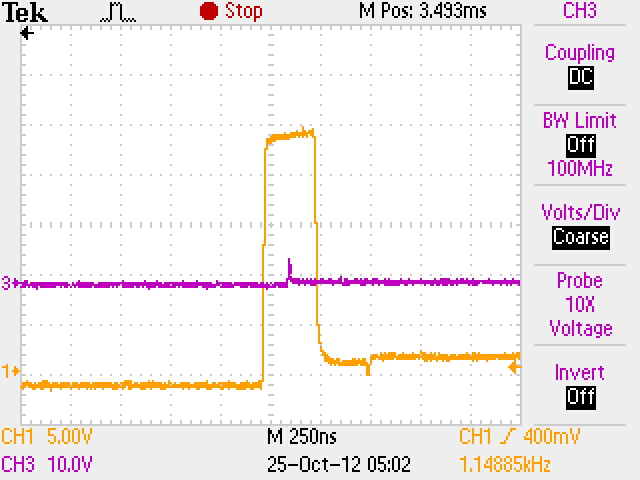
\includegraphics[scale=0.3]{CC2.jpg}
\caption{Courbes obtenus à l'oscilloscope pour le projet 3 en utilisant une charge complexe}
\label{CC2}
\end{center}
\end{figure}

\subsection*{Calcul de R}
En identifiant la valeur finale de la tension (après quelques constantes de temps), on peut déduire la valeur de R conaissant $V^{+}$  et $Z_0$. On utilise l'équation suivante:
\begin{equation}
V_{finale} = V^{+} \left( 1 + \frac{R - Z_0}{R + Z_0}\right)
\end{equation}

On a que $V_{finale} = 3V et Z_0 = 50 \Omega$. On développe l'équation:

\begin{align*}
V_{finale} &= V^{+} \left( 1 + \frac{R - Z_0}{R + Z_0}\right)\\
3 &= 14 \left( 1 + \frac{R - 50}{R + 50}\right)\\
R &= 6 \Omega
\end{align*}

\subsection*{Calcul de $\tau$}

Conaissant maintenant R, on peut trouver $\tau$ au moyen d'un point dans la pente descendante de la courbe, selon l'équation suivante:
\begin{equation}
V_{t\leq \tau} = V^{+} \left( \left(1 + \frac{R - Z_0}{R + Z_0}\right) + \left(1 -\frac{R - Z_0}{R + Z_0}\right) e^{-t/\tau} \right)
\end{equation}

Pour $R=6 \Omega$, $Z_0 = 50 \Omega$ et $V_{t= 250ns} = 16$, on développe l'équation précédente:

\begin{align*}
16 &= 14 \left( \left(1 + \frac{6 - 50}{6 + 50}\right) + \left(1 -\frac{6 - 50}{6 + 50}\right) e^{-250 \times 10^{-9}/\tau} \right)\\
0.5102 &= e^{-250 \times 10^{-9}/\tau}\\
\tau   &= \frac{1}{\frac{ln(0.5102)}{-250 \times 10^{-9}}}\\
\tau   &= 371.497\left[ns\right]
\end{align*}

\subsection*{Calcul de L}

Conaissant maintenant $\tau$, on peut déterminer l'inductance L au moyen de l'équation suivante:
\begin{equation}
\tau = \frac{L}{R + Z_0}
\end{equation}
Pour $R = 6 \Omega$, $Z_0 = 50 \Omega$ et $\tau = 371.497\left[ns\right]$, on développe l'équation précédente:
\begin{align*}
371.497\times 10^{-9} &= \frac{L}{6 + 50}\\
L = 20.8 \left[\mu H\right]
\end{align*}
\newpage
\section{Projet 4}
\subsection{Tracé des régimes transitoires à l'oscilloscope}
Nous avons réalisé le montage pratique tel qu'illustré à la figure 4 de l'énoncé de laboratoire. L'ordre des lignes de transmission a été respecté. Le tracé (à l'oscilloscope) des réponses transitoires obtenues pour des impédances de respectivement 0 $\Omega$, 50 $\Omega$ et 100 $\Omega$ sont présentées aux figures ci-dessous. Il est à noté que le signal vu de la source est sur le canal 1 (orange), que le signal vu à la jonction entre les deux lignes est sur le canal 2 (bleu) et que le signal vu de la charge est sur le canal 3 (vert).

\begin{figure}[htb]
	\centering
\subfigure[Régime transitoire vu de la source, à la jonction entre les lignes et à la charge pour $R = 0 \Omega$]{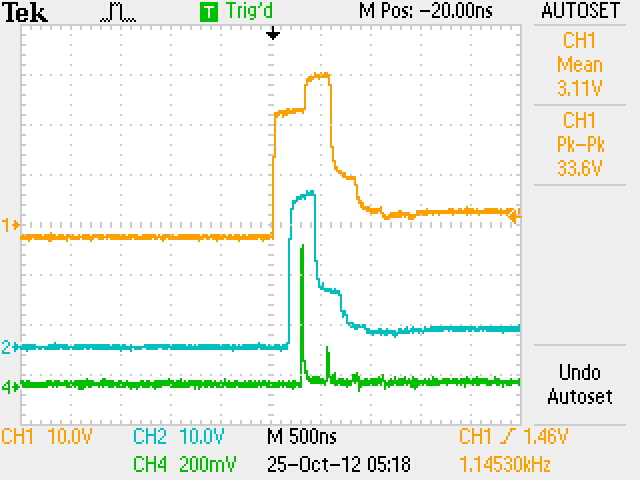
\includegraphics[scale =0.3]{fig/2CRC.JPG} \label{fig:trans2r0}}
		\quad
		\subfigure[Régime transitoire vu de la source, à la jonction entre les lignes et à la charge pour $R = 50 \Omega$]{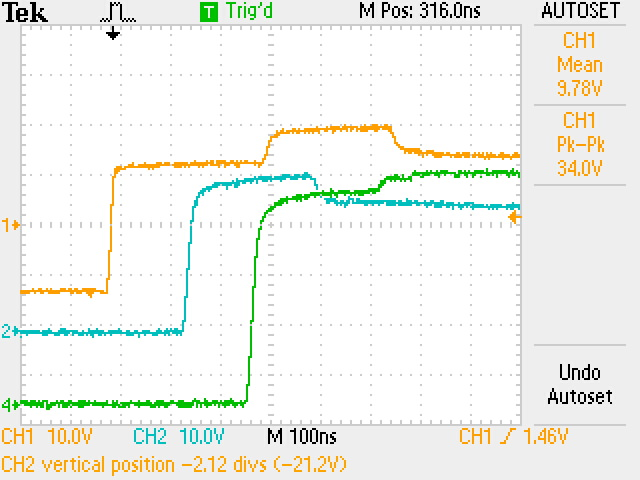
\includegraphics[scale =0.3]{fig/2CR50.JPG} \label{fig:trans2r50}}
		\quad
		\subfigure[Régime transitoire vu de la source, à la jonction entre les lignes et à la charge pour $R = 100 \Omega$]{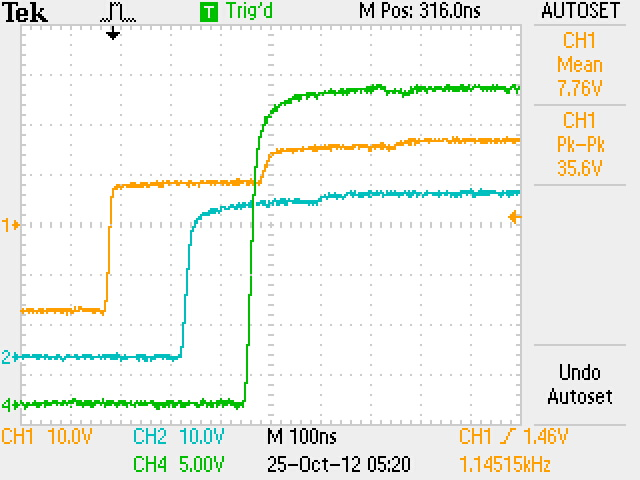
\includegraphics[scale =0.3]{fig/2CR100.JPG} \label{fig:trans2r100}}
\end{figure}
\newpage
\subsection{Calcul du coefficient de réflexion à la source}
Pour calculer le coefficient de réflexion à la source, on utilise l'équation \ref{eq:reflex} en sachant qu'elle sera la même peu importe la charge:
\begin{align*}
\Gamma_g (s) &= \frac{50 - 50}{50 + 50}\\
&= 0
\end{align*}
\subsection{Calcul du coefficient de réflexion du côté de la ligne \# 1}
On définit l'équation suivante et on la développe selon les valeurs connues
\begin{align}
\Gamma_{11} &= \frac{Z_{02} - Z_{01}}{Z_{02} + Z_{01}}\\
			&= \frac{93-50}{93 + 50}\notag\\
			&= 0.3007\notag
\end{align}
\subsection{Calcul du coefficient de réflexion du côté de la ligne \# 2}
On définit l'équation suivante et on la développe selon les valeurs connues
\begin{align}
\Gamma_{22} &= \frac{Z_{01} - Z_{02}}{Z_{01} + Z_{02}}\\
			&= \frac{50-93}{93 + 50}\notag\\
			&= -0.3007\notag
\end{align}
\subsection{Calcul des coefficients de réflexion du côté des charges}
\textbf{Pour R = $0\Omega$}
\begin{align*}
\Gamma_c (s) &= \frac{Z_c(s) - Z_0(s)}{Z_c(s) + Z_0(s)}\\
			 &= \frac{0 - 93 }{0 + 93}\\
			 &= -1
\end{align*}
\textbf{Pour R = $50\Omega$}
\begin{align*}
\Gamma_c (s) &= \frac{Z_c(s) - Z_0(s)}{Z_c(s) + Z_0(s)}\\
			 &= \frac{50 - 93 }{93 + 50}\\
			 &= -0.3007
\end{align*}
\textbf{Pour R = $100\Omega$}
\begin{align*}
\Gamma_c (s) &= \frac{Z_c(s) - Z_0(s)}{Z_c(s) + Z_0(s)}\\
			 &= \frac{100 - 93 }{100 + 93}\\
			 &= 0.0363
\end{align*}
\subsection{Calcul du coefficient de transmission de la ligne \# 1 vers la ligne \# 2}
On définit l'équation suivante et on la développe selon les valeurs connues
\begin{align}
\tau_{12} &= (1-\Gamma_{11})\\
			&= 1 - 0.3007\notag\\
			&= 0.6993\notag
\end{align}
\subsection{Calcul du coefficient de transmission de la ligne \# 2 vers la ligne \# 1}
On définit l'équation suivante et on la développe selon les valeurs connues
\begin{align}
\tau_{21} &= (1-\Gamma_{22})\\
			&= 1 + 0.3007\notag\\
			&= 1.3007\notag
\end{align}
\subsection{Régimes transitoires théoriques }

\begin{figure}[htb]
	\centering
\mbox{\subfigure[Régime transitoire théorique vu de la source, à la jonction entre les lignes et à la charge pour $R = 0 \Omega$]{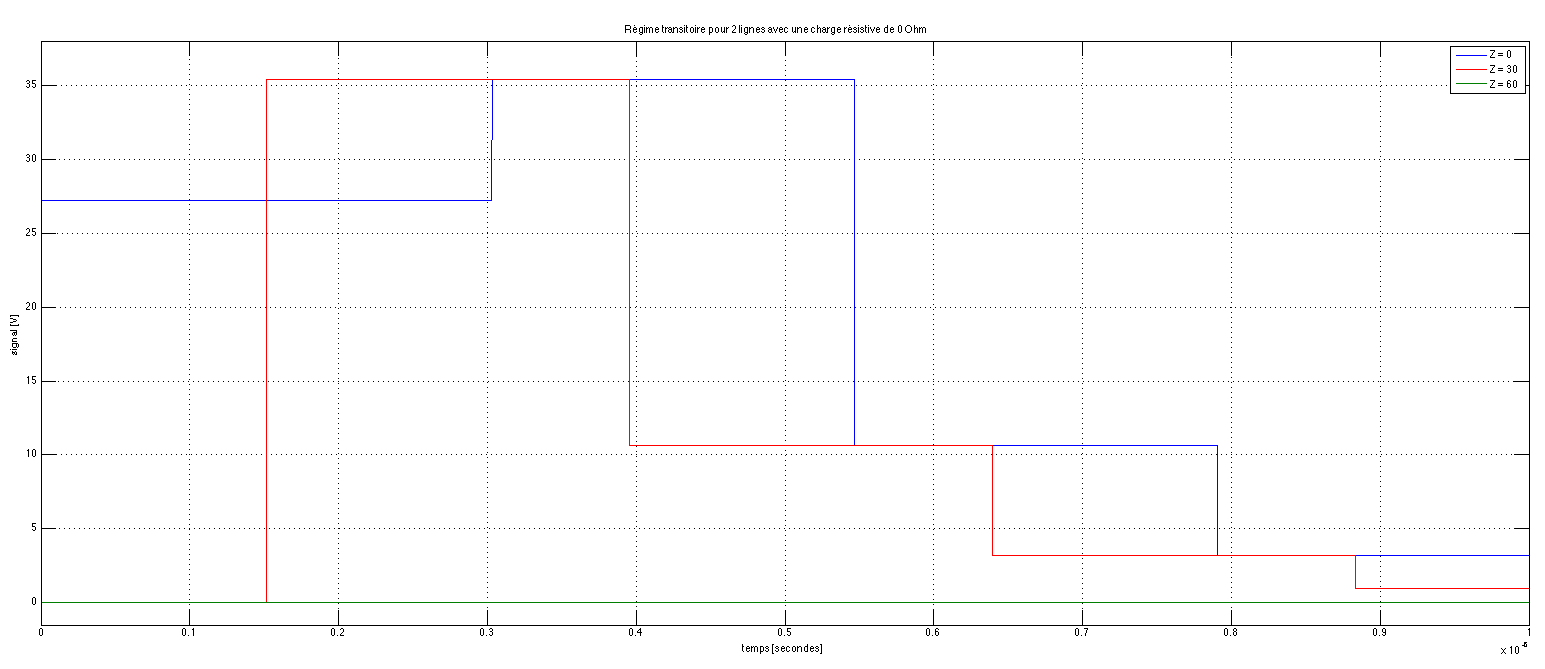
\includegraphics[scale =0.3]{fig/2r0.png} \label{fig:2r0}}}
\end{figure}



\begin{figure}[htb]
	\centering
	\mbox{\subfigure[Régime transitoire théorique vu de la source, à la jonction entre les lignes et à la charge pour $R = 50 \Omega$]	{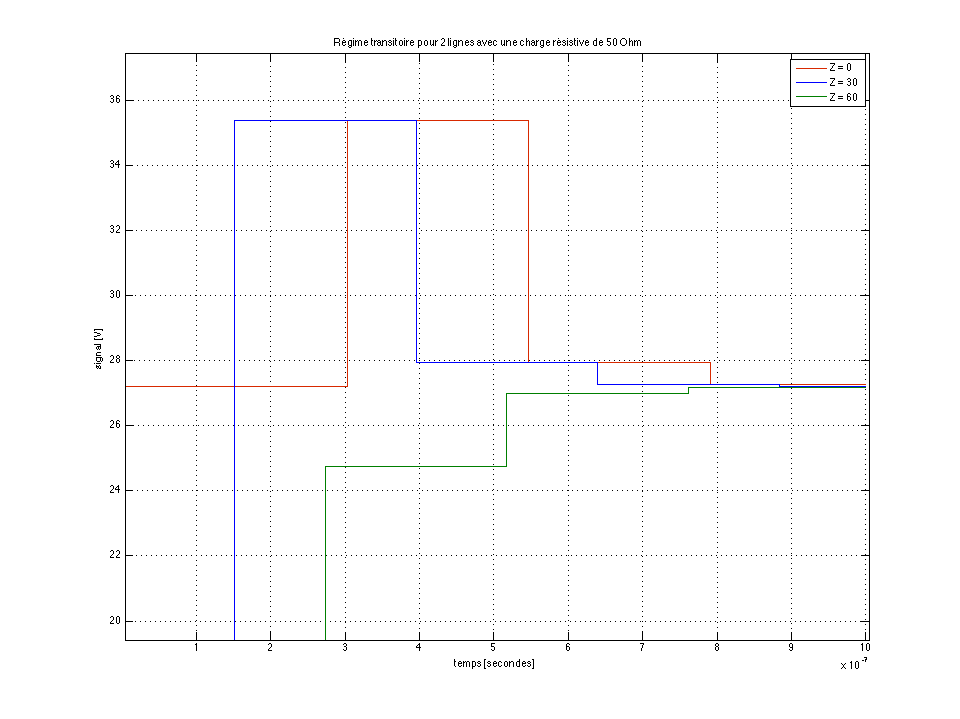
\includegraphics[scale =0.25]{fig/2r50.png} \label{fig:2r50}}
		\subfigure[Régime transitoire théorique vu de la source, à la jonction entre les lignes et à la charge pour $R = 100 \Omega$]{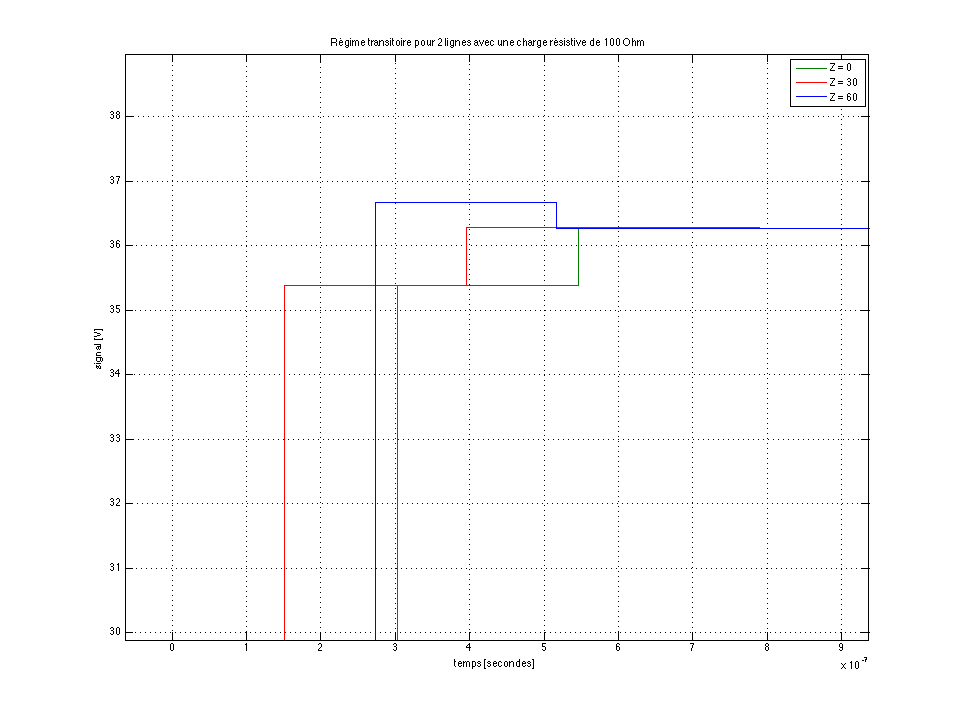
\includegraphics[scale =0.25]{fig/2r100.png} \label{fig:2r100}}}
\end{figure}


\subsection{Diagrammes en z}

\begin{figure}[htb]
	\centering
	\mbox{\subfigure[Diagramme en z pour $R = 0 \Omega$]{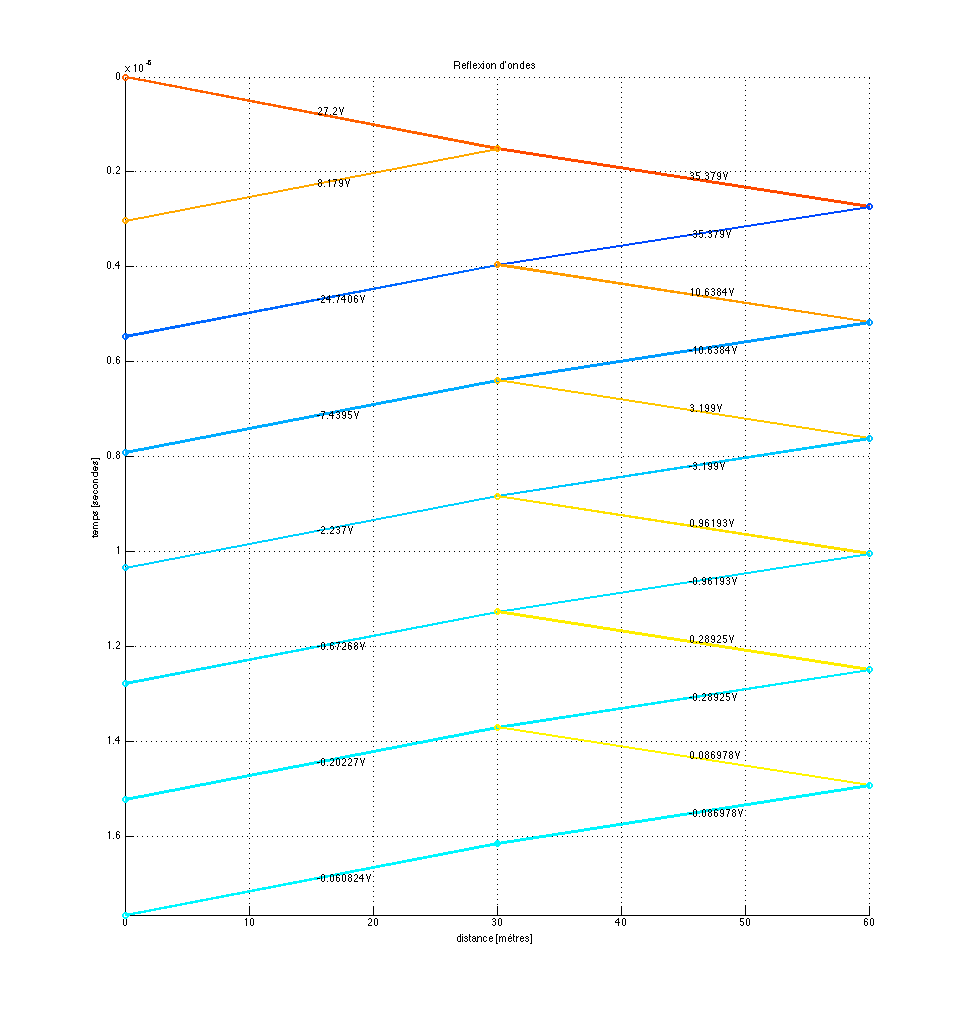
\includegraphics[scale =0.25]{fig/2zr0.png} \label{fig:2zr0}}
		\subfigure[Diagramme en z pour $R = 50 \Omega$]{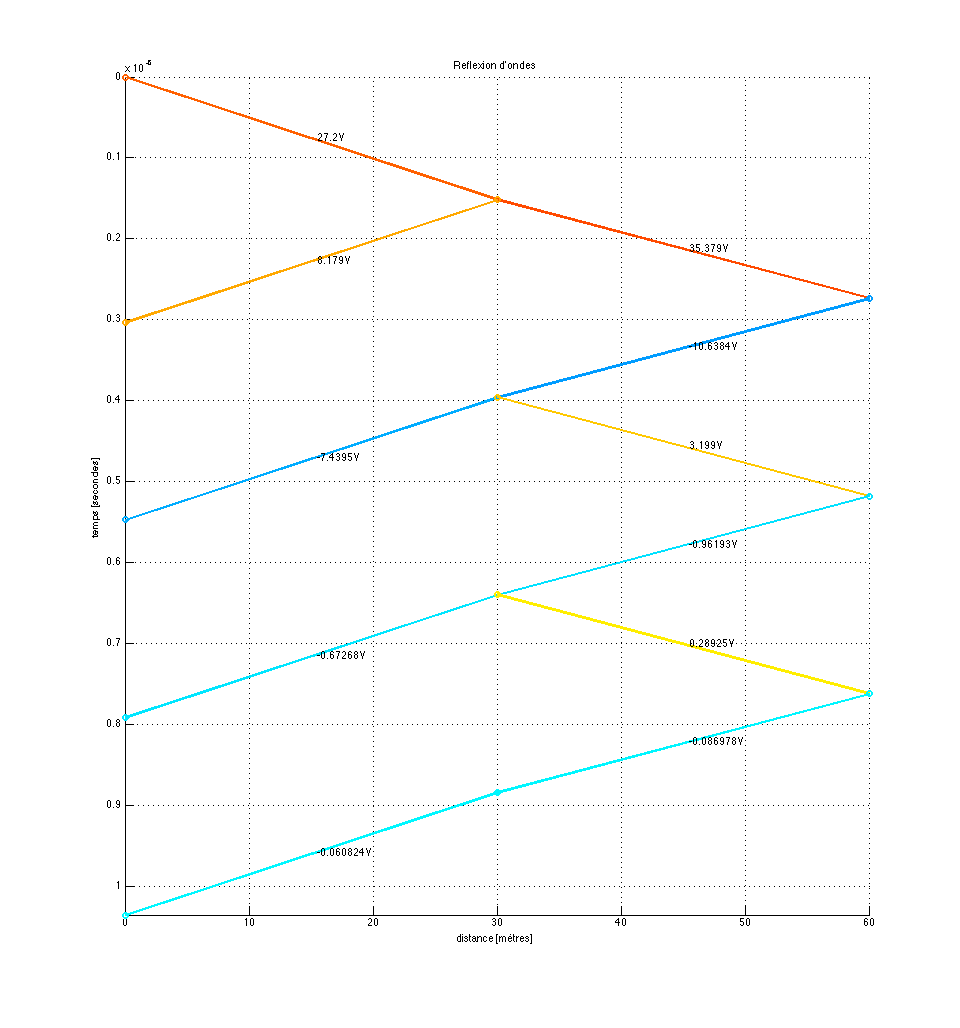
\includegraphics[scale =0.25]{fig/2zr50.png} \label{fig:2zr50}}}
\end{figure}
\begin{figure}[htb]
	\centering
	\mbox{\subfigure[Diagramme en z pour $R = 100 \Omega$]{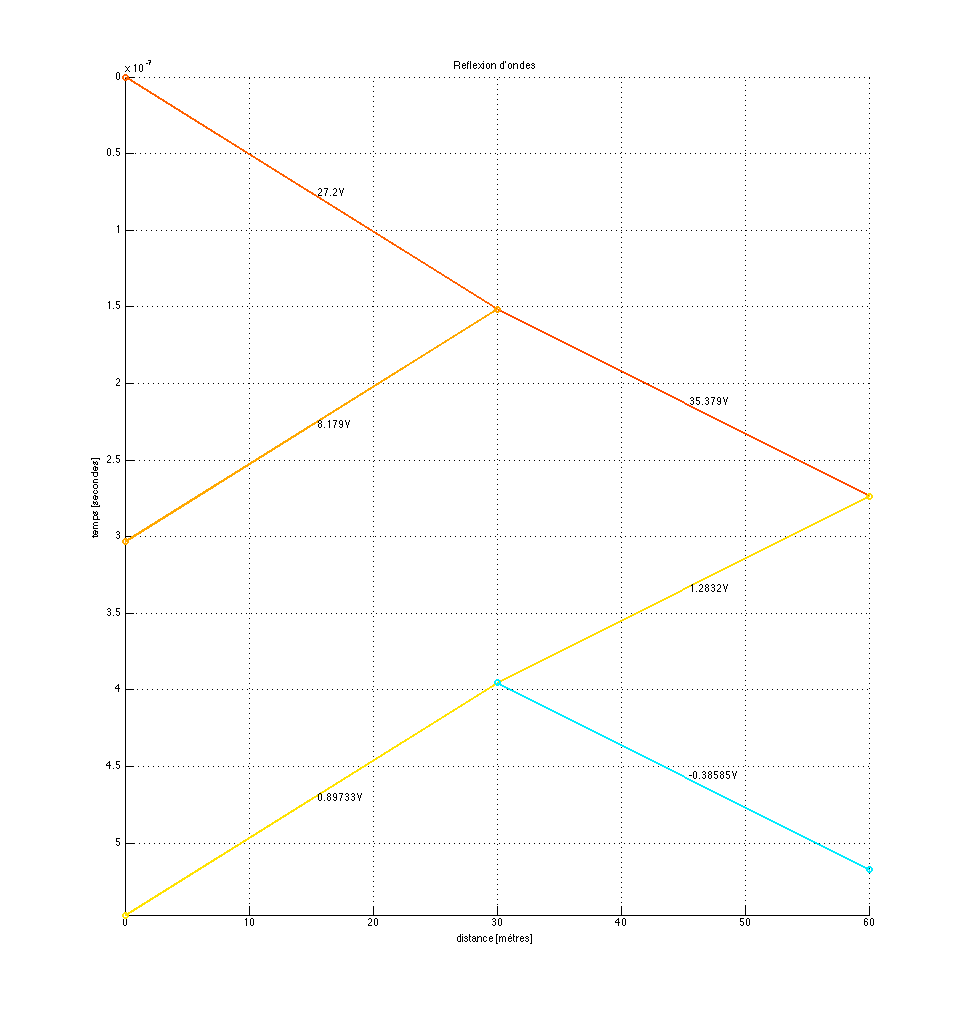
\includegraphics[scale =0.25]{fig/2zr100.png} \label{fig:2zr100}}}
\end{figure}
\clearpage
\newpage

\subsection{Discussion}
